%\documentclass{article}
\documentclass[class=minimal,border=4pt]{standalone}
\usepackage{tikz}
\usetikzlibrary{patterns}
\newcommand\actfill{1.0}
\newcommand\actcol{yellow}
\newcommand\tikscale{0.32}
\newcommand{\smiley}{\tikz[baseline=-0.75ex,black]{
\filldraw[fill=orange!10] circle (2mm);
\node[fill,circle,inner sep=0.5pt] (left eye) at (135:0.8mm) {};
\node[fill,circle,inner sep=0.5pt] (right eye) at (45:0.8mm) {};
\draw[-] (-145:0.9mm) arc (-120:-60:1.5mm);
}
}
\newcommand{\frownie}{\tikz[baseline=-0.75ex,black]{
\filldraw[fill=red!20] circle (2mm);
\node[fill,circle,inner sep=0.5pt] (left eye) at (135:0.8mm) {};
\node[fill,circle,inner sep=0.5pt] (right eye) at (45:0.8mm) {};
\draw[-] (-145:0.9mm) arc (120:60:1.5mm);
}
}

\pgfdeclarepatternformonly{dark lines}{\pgfqpoint{-1pt}{-1pt}}{\pgfqpoint{12pt}{12pt}}{\pgfqpoint{12pt}{12pt}}%
{
  \pgfsetlinewidth{3pt}
  \pgfpathmoveto{\pgfqpoint{0pt}{0pt}}
  \pgfpathlineto{\pgfqpoint{12pt}{12pt}}
  \pgfusepath{stroke}
}

   
\begin{document}
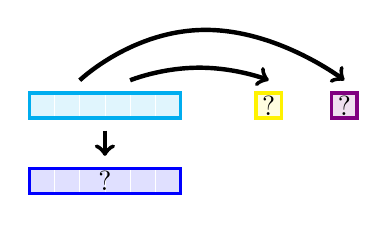
\begin{tikzpicture}[
fill opacity=.6,draw opacity=1,scale=\tikscale,
emptynode/.style={square}
]
\fill[fill=cyan!20, very thick] (0,0) rectangle (6,1);
\draw[ystep=1cm,xstep=1cm,white,very thin] (0,0) grid (6,1);
\draw[color=cyan, very thick] (0,0) rectangle (6,1);

\fill[fill=yellow!20, very thick] (9,0) rectangle (10,1);
%\draw[ystep=1cm,xstep=1cm,white,very thin] (9,0) grid (10,1);
\draw[color=yellow, very thick] (9,0) rectangle (10,1);
\node at (9.5,0.5) [fill opacity=1,color=black] {?};

\fill[fill=violet!20, very thick] (12,0) rectangle (13,1);
%\draw[ystep=1cm,xstep=1cm,white,very thin] (9,0) grid (13,1);
\draw[color=violet, very thick] (12,0) rectangle (13,1);
\node at (12.5,0.5) [fill opacity=1,color=black] {?};

\draw[black,ultra thick,->] plot[smooth,tension=1] coordinates {(4.0,1.5) (6.75, 2.0) (9.5,1.5)};
\draw[black,ultra thick,->] plot[smooth,tension=1] coordinates {(2.0,1.5) (7.0, 3.5) (12.5,1.5)};

\fill[fill=blue!20, very thick] (0,-3) rectangle (6,-2);
\draw[ystep=1cm,xstep=1cm,white,very thin] (0,-3) grid (6,-2);
\draw[color=blue, very thick] (0,-3) rectangle (6,-2);
\node at (3,-2.5) [fill opacity=1,color=black] {?};
\draw[black,ultra thick,->] plot[smooth,tension=1] coordinates {(3.0,-0.5) (3.0,-1.5)};

\end{tikzpicture}
\end{document}

